%%%%%%%%%%%%%%%%%%%%%%%%%%%%%%%%%%%%%%%%%
% University Assignment Title Page 
% LaTeX Template
% Version 1.0 (27/12/12)
%
% This template has been downloaded from:
% http://www.LaTeXTemplates.com
%
% Original author:
% WikiBooks (http://en.wikibooks.org/wiki/LaTeX/Title_Creation)
%
% License:
% CC BY-NC-SA 3.0 (http://creativecommons.org/licenses/by-nc-sa/3.0/)
% 
% Instructions for using this template:
% This title page is capable of being compiled as is. This is not useful for 
% including it in another document. To do this, you have two options: 
%
% 1) Copy/paste everything between \begin{document} and \end{document} 
% starting at \begin{titlepage} and paste this into another LaTeX file where you 
% want your title page.
% OR
% 2) Remove everything outside the \begin{titlepage} and \end{titlepage} and 
% move this file to the same directory as the LaTeX file you wish to add it to. 
% Then add \input{./title_page_1.tex} to your LaTeX file where you want your
% title page.
%
%%%%%%%%%%%%%%%%%%%%%%%%%%%%%%%%%%%%%%%%%

%----------------------------------------------------------------------------------------
%	PACKAGES AND OTHER DOCUMENT CONFIGURATIONS
%----------------------------------------------------------------------------------------

\documentclass[12pt]{article}
\usepackage[utf8]{inputenc}
\usepackage[french]{babel}
\usepackage[babel=true]{csquotes}
\usepackage{bold-extra}
\usepackage{lmodern,textcomp}


%%%%%%\usepackage{hyperref}
%\usepackage[super,square]{natbib}

%% BIBTEX %%
\usepackage[backend=biber, sorting=none, style=numeric, natbib=true]{biblatex}
\DeclareCiteCommand{\supercite}[\mkbibsuperscript]
  {\iffieldundef{prenote}
     {}
     {\BibliographyWarning{Ignoring prenote argument}}%
   \iffieldundef{postnote}
     {}
     {\BibliographyWarning{Ignoring postnote argument}}}
  {\usebibmacro{citeindex}%
   \bibopenbracket\usebibmacro{cite}\bibclosebracket}
  {\supercitedelim}
  {}
\let\citep=\supercite
%\usepackage[round]{natbib}
%\addbibresource{finite_state_machine.bib}
\bibliography{protocole}
%%

%% Centrer de grand tableau et figures %%
\usepackage{adjustbox}
\usepackage{array,multirow,makecell,tabularx}
\setcellgapes{1pt}
\makegapedcells
%\newcolumntype{R}[1]{>{\raggedleft\arraybackslash }b{#1}}
%\newcolumntype{L}[1]{>{\raggedright\arraybackslash }b{#1}}
%\newcolumntype{C}[1]{>{\centering\arraybackslash }b{#1}}
\newcolumntype{C}{>{\centering}X}
%%

\usepackage{longtable}
\usepackage{graphicx} 
\usepackage{xifthen}
\usepackage{tabularx}
\usepackage{adjustbox}
\usepackage{amsmath}
%\usepackage[clean,pdf]{svg}
\usepackage{pdfpages}
\usepackage[unicode,hidelinks]{hyperref}
\usepackage[]{url}
%\usepackage{tablefootnote}
\usepackage{footnote}
%\usepackage[bottom]{footmisc}
%\makesavenoteenv{tabular}
\makesavenoteenv{table}
\makesavenoteenv{tabularx}

%\usepackage[super,square]{natbib}

%\newenvironment{agrandirmarges}[2]{%
%\begin{list}{}{%
%\setlength{\topsep}{0pt}%
%\setlength{\listparindent}{\parindent}%
%\setlength{\itemindent}{\parindent}%
%\setlength{\parsep}{0pt plus 1pt}%
%\ifthenelse{\isodd{\value{page}}}%
%{\setlength{\leftmargin}{-#1}\setlength{\rightmargin}{-#2}}
%{\setlength{\leftmargin}{-#2}\setlength{\rightmargin}{-#1}}
%}\item }%
%{\end{list}}



\usepackage[nottoc, notlof, notlot]{tocbibind}

\usepackage[left=4.2cm,right=4.2cm,top=3.5cm,bottom=3.5cm]{geometry}

\newcommand{\doctitle}{Protocole de synchronisation décentralisé}
\newcommand{\authorName}{Olivier \textsc{Radisson}}
\usepackage{fancyhdr}
\pagestyle{fancy}
\lhead{\doctitle}
\rhead{\authorName}
%\lfoot{Document réalisé par l'équipe n$^\circ$4}
\renewcommand{\headrulewidth}{0.4pt}
\renewcommand{\footrulewidth}{0.4pt}
\renewcommand{\newline}{~\\~\\}
\newcommand{\p}{\newline \indent}
\newcommand{\rt}{~\\ \indent}
\newcommand{\centergraph}[3][]{\begin{center}%
\begin{figure}[h!]%
\vspace{-5pt}%
\centerline{\includegraphics[width=#3]{#2}}%
\ifthenelse{\isempty{#1}}{}{\vspace{-8pt}\caption{#1}}%
\vspace{-5pt}%
\label{#2}%
\end{figure}%
\end{center}}
\newcommand{\newparagraph}{~\\\indent}

\setcounter{secnumdepth}{3}
%\setcounter{tocdepth}{2}


\begin{document}




\begin{titlepage}

\newcommand{\HRule}{\rule{\linewidth}{0.5mm}} % Defines a new command for the horizontal lines, change thickness here

\center % Center everything on the page
 
%----------------------------------------------------------------------------------------
%	HEADING SECTIONS
%----------------------------------------------------------------------------------------

\textsc{\LARGE Institut National des Sciences Appliquées de Lyon\\
\&\vspace{10pt}~
\\KompleXKapharnaüM}\\[1.0cm] % Name of your university/college
\textsc{\small Stage de 4\up{ème} année du département Génie Électrique} \\[0.2cm]
\textsc{\Large Projet Do Not Clean}
\\[0.5cm] % Major heading such as course name
\textsc{\large Réalisation d'une carte multimédia programmable et contrôlable via wifi}\\[0.5cm] % Minor heading such as course title

%----------------------------------------------------------------------------------------
%	TITLE SECTION
%----------------------------------------------------------------------------------------

\HRule \\[0.4cm]
%{ \huge  \textsc{\textbf{Plan Projet}}}\\[0.4cm] % Title of your document
{ \huge   \scshape{\doctitle}  } % \bfseries
\HRule \\[1.5cm]
 
%----------------------------------------------------------------------------------------
%	AUTHOR SECTION
%----------------------------------------------------------------------------------------

\begin{minipage}{0.4\textwidth}
\begin{flushleft} \large
\emph{Auteur:}\\
Olivier \textsc{Radisson}\\
~ \\
~ \\
~ \\
~ \\
\end{flushleft}
\end{minipage}
~
\begin{minipage}{0.4\textwidth}
\begin{flushright} \large
\emph{Tuteur de stage :} \\
Gilles \textsc{Gallet}
~ \\
~ \\
\emph{Chef de projet :} \\
Pierre \textsc{Hoezelle}
~ \\
~ \\

\end{flushright}
\end{minipage}\\[1.5cm]

% If you don't want a supervisor, uncomment the two lines below and remove the section above
%\Large \emph{Author:}\\
%John \textsc{Smith}\\[3cm] % Your name

%----------------------------------------------------------------------------------------
%	DATE SECTION
%----------------------------------------------------------------------------------------
\vspace{2.2cm}
{\large - 8 janvier 2015 -}\\ \vspace{10pt}
{\large Dernière édition le \today}\\
%{\large  ~~~ : \today}\\[3cm] % Date, change the \today to a set date if you want to be precise

%----------------------------------------------------------------------------------------
%	LOGO SECTION
%----------------------------------------------------------------------------------------

%\includegraphics{Logo}\\[1cm] % Include a department/university logo - this will require the graphicx package
 
%----------------------------------------------------------------------------------------

\vfill % Fill the rest of the page with whitespace

\end{titlepage}


%\newpage
%~
%	\thispagestyle{empty}
    

\newpage
\thispagestyle{empty}
\begin{abstract}
Ce document présente le protocole de synchronisation qui est la base du réseau décentraliser des cartes.\\
Ce protocole s'occupe de synchroniser entre les cartes : 
\begin{itemize}
\item La liste des cartes présente, leur nom et l'adresse IP associé
\item Le temps sous forme d'un \textit{timetag}
\item La version globale du scénario
\end{itemize}~\\
\indent Le protocole est exécuté par chaque carte via une Machine à nombre Fini d'États\citep{document_ImplementationdesMachinesanombreFinidEtats_} qui sera l'objet principal de ce document avec la liste des messages OSC associés.\p
Ce document présente aussi rapidement le protocole ACK créé pour l'occasion qui est une surcharge de l'OSC permettant de s'assurer qu'un message est bien parvenu à destination.




\end{abstract}

\newpage
~ \thispagestyle{empty}
%\newpage
%\thispagestyle{empty}

\tableofcontents

%\newpage
%~ \thispagestyle{empty}
\newpage

\setcounter{page}{1}

\section{Introduction}
\textit{Ce document à une visée majoritairement technique. Les points abordés peuvent intéresser les utilisateurs les plus curieux, mais sa vocation première est de présenter le fonctionnement du protocole de synchronisation pour documenter le développement}\p
Les cartes électronique crées dans le cadre du stage pour le projet Do Not Clean sont des cartes reliées à un réseau informatique via un signal WIFI\citep{encyclopediaArticle_WiFi_}. Il a été explicitement demandé que ces cartes puissent communiquer entre elles et former un réseau, mais sans nécessité la présence d'un élément central ou d'une régie.\p
De plus ces cartes doivent partager entre elles un certains nombre d'information dont les principales sont : \begin{itemize}
\item Le temps
\item Le scénario à jouer
\item La liste des cartes présentes
\end{itemize}
C'est pour répondre à ce besoin que le protocole décrit ci-dessous à été inventé.\p
Pour assurer un fonctionnement le plus robuste possible malgré l'utilisation d'une connexion WIFI et du protocole UDP\citep{webpage_UserDatagramProtocol_Postela} pour le transport des données, il a été également inventé un petit protocole d'\textit{acknwolegment} dénommé ACK qui s'assure qu'un message a bien été reçu.


\section{Présentation du protocole ACK}
Le protocole ACK est une sur-couche du protocole OSC\footnote{\textit{Open Sound Control}}\citep{webpage_TheOpenSoundControl10Specificationopensoundcontrolorg_} qui s'assure de la bonne réception d'un message.\p
L'émetteur du message OSC ajoute en début de celui-ci deux nouvelles informations permettant d'identifier ne manière unique le message. Ensuite il envoi celui-ci au destinataire sur un port différent que celui prévu pour les communication OSC classique.\\
Tant que l'émetteur n'a pas reçu de confirmation de réception il envoie le même message autant de fois qu'il lui est défini de faire.\p
Lorsque le destinataire reçoit un message sur ce port il vérifie si celui-ci n'a pas déjà été reçus et ce grâce aux deux identifiants uniques. Si le message est reçu pour la première fois celui-ci est transmit à la couche supérieur comme s'il s'agissait d'un message OSC classique. Si le message avait déjà été reçus il est simplement ignoré. \\
Enfin, dans tous les cas le destinataire renvoie quoi qu'il en soit un message, avec les mêmes identifiants, à l'émetteur pour lui signifier qu'il a bien reçu le message.\p
Une fois que l'émetteur a reçu confirmation de la réception de son message il arrête d'envoyer en série le message et peut être sur que celui-ci est bien arrivé.

\subsection{Empaquetage d'une trame OSC via le protocole ACK} 
\begin{table}[htbp]
\centering
{
\textbf{Trame OSC via le protocole ACK}\vspace{8pt}~\\
\begin{tabularx}{0.85\textwidth}{|c|c|c|C|}
\hline
\textbf{IP} & \textbf{Port} & \textbf{Protocole} & \textbf{Adresse}  \tabularnewline
\hline
\hline
X.X.X.X & 1782 & UDP & $\cdots$ \tabularnewline
\hline
\end{tabularx}
\vspace{10pt}
~\\\textbf{Arguments}\vspace{5pt}\\
}
\begin{adjustbox}{center}
\small
\begin{tabularx}{0.65\textwidth}{|c||c|C|}
\hline
\textbf{Champs} & \textbf{Type} & \textbf{Valeur}  \tabularnewline
\hline
\hline
ID\_time & int & {\tiny\fontfamily{ccr}\selectfont (0xFFFF0000 \& \textit{time.tv\_sec}) $\mid$ ((0xFFFF0000 \& \textit{time.tv\_nsec}) $\gg$ 16)} \tabularnewline
\hline
ID\_rand & int & \texttt{rand()}  \tabularnewline
\hline
$\cdots$ & $\cdots$ & $\cdots$ \tabularnewline
\hline
\end{tabularx}
\normalsize
\end{adjustbox}
\label{tab:trame_osc_ack}
\caption{Trame OSC générique pour un message transporté par le protocole ACK}
\vspace{-5pt}
\end{table}
\indent Un message OSC quelconque se verra empaqueté de cette manière avec les deux identifiants unique \texttt{ID\_time} et \texttt{ID\_rand}.\\
L'adresse ainsi que le reste des arguments sont remplies par le message d'origine.

\subsection{Message de réponse}
À chaque fois qu'une carte reçoit un message sur le port définit pour le protocole ACK il répond via le message présenté par la table \ref{tab:trame_ack} pour signifier que le message lui est bien parvenu\footnote{Chaque message excepté bien-sûr un message sur l'adresse \textit{/ack}}.
\begin{table}[htbp]
\centering
{
\textbf{Trame OSC}\vspace{8pt}~\\
\begin{tabularx}{0.85\textwidth}{|c|c|c|C|}
\hline
\textbf{IP} & \textbf{Port} & \textbf{Protocole} & \textbf{Adresse}  \tabularnewline
\hline
\hline
X.X.X.X & 1782 & UDP & /ack \tabularnewline
\hline
\end{tabularx}
\vspace{10pt}
~\\\textbf{Arguments}\vspace{5pt}\\
}
\begin{adjustbox}{center}
\small
\begin{tabularx}{0.65\textwidth}{|c||c|C|}
\hline
\textbf{Champs} & \textbf{Type} & \textbf{Valeur}  \tabularnewline
\hline
\hline
ID\_time & int & \textit{ID\_time} \tabularnewline
\hline
ID\_rand & int & \textit{ID\_rand}  \tabularnewline
\hline
\end{tabularx}
\normalsize
\end{adjustbox}
\label{tab:trame_ack}
\caption{Trame OSC pour signifier la réception d'un message ACK}
\vspace{-5pt}
\end{table}

\section{Protocole de synchronisation décentralisé}

Le protocole qui va permettre de synchroniser chaque carte avec le reste du réseau de manière décentralisé se base sur l'émission d'un court message de présentation sur l'adresse de broadcast\footnote{L'adresse de broadcast est une adresse de destination tel que tous les éléments d'un même réseau prennent le message comme leur étant adressé. Ceci permet de communiquer avec des éléments du réseau sans connaître leur adresse IP.} et à intervalle régulier.\p
Ce message de présentation inclus le nom unique de la carte qui l'émet ainsi que son \textit{timetag}\footnote{Le \textit{timetag} représente une référence de temps absolue que possède la carte. Cette notion sera développé plus en détails plus tard.} et la version du scénario dont il dispose. Chaque carte qui reçoit un message de ce type ajoute, si ce n'est pas déjà le cas, la carte qui l'a émit dans sa liste des cartes présente.\\
Ensuite elle vérifie si son \textit{timetag} n'est pas plus vieux que le sien, si c'est le cas il y aura demande de synchronisation. De même pour la version du scénario.\p
Ce fonctionnement totalement décentralisé permet une grande souplesse dans la structure de réseau et surtout la création de sous réseau si la connexion est perdue puis le regroupement en un seul grand réseau lorsque la connexion est rétablie et ce, de manière toute à fait transparente.

\subsection{Présentation sur le réseau}

À intervalle régulier et définie en avance. Chaque carte du réseau va envoyer un message de présentation sur l'adresse de broadcast.

\subsubsection{Trame OSC de présentation}

La trame pour se présenter est la suivant :

\begin{table}[htbp]
\centering
{
\textbf{Trame OSC}\vspace{8pt}~\\
\begin{tabularx}{0.85\textwidth}{|c|c|c|C|}
\hline
\textbf{IP} & \textbf{Port} & \textbf{Protocole} & \textbf{Adresse}  \tabularnewline
\hline
\hline
255.255.255.255 & 1781 & UDP & /iamhere \tabularnewline
\hline
\end{tabularx}
\vspace{10pt}
~\\\textbf{Arguments}\vspace{5pt}\\
}
\begin{adjustbox}{center}
\small
\begin{tabularx}{0.65\textwidth}{|c||c|C|}
\hline
\textbf{Champs} & \textbf{Type} & \textbf{Valeur}  \tabularnewline
\hline
\hline
uName & string & \textit{Nom unique de la carte} \tabularnewline
\hline
timetag & int & \textit{Temps de référence}  \tabularnewline
\hline
scenario & int & \textit{Version du scénario}  \tabularnewline
\hline
\end{tabularx}
\normalsize
\end{adjustbox}
\label{tab:trame_iamhere}
\caption{Trame OSC pour signifier sa présence sur le réseau}
\vspace{-5pt}
\end{table}~\\
\indent Chaque élément de réseau recevant ce message va vérifier s'il ne connait pas déjà la carte en question. Si celle-ci est nouvelle il l'ajoute dans sa table des cartes présentes sur le réseau.\\
Ensuite si le timetag de l'émetteur est plus récent il va demander une synchronisation du temps, si il est inférieur il va lui envoyer un message de présentation pour forcer celui-ci à lui demander en retour une synchronisation du temps\footnote{Il n'y a comme cela toujours que l'élément en retard qui provoque une synchronisation du temps, cela rends plus simple le protocole.}. Il en va de même pour la version du scénario.

\subsubsection{FSM de la partie présentation du protocole}
Voici la FSM partielle correspondant à la partie présentation sur le réseau :
\begin{figure}[htbp]
  \centering
  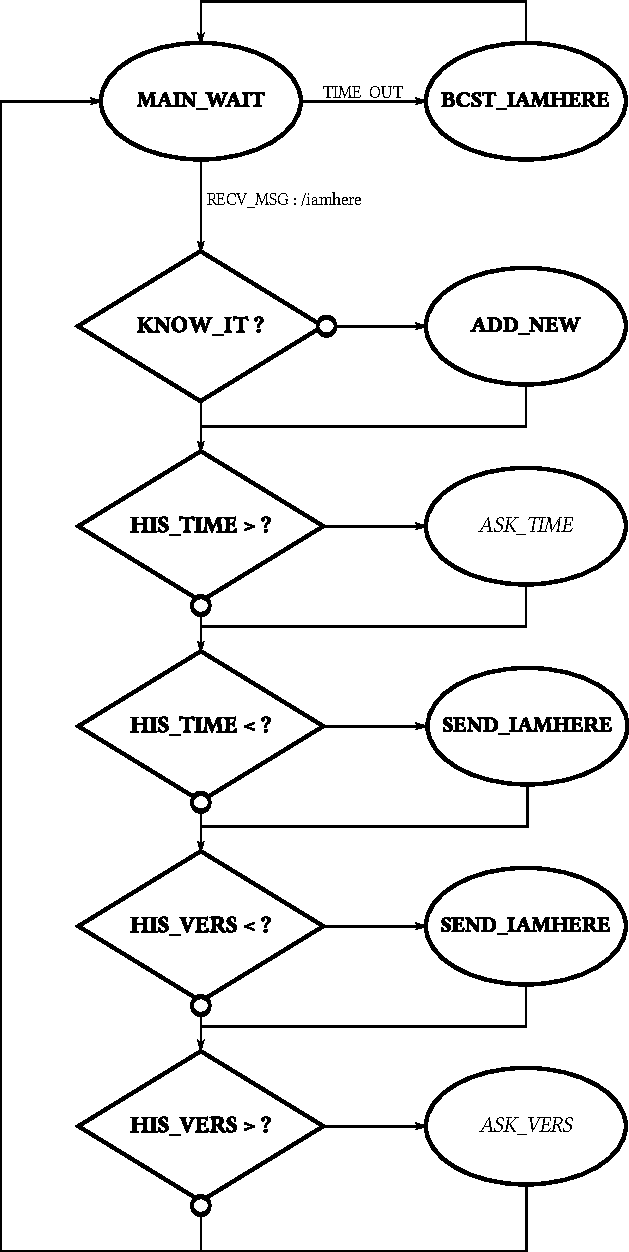
\includegraphics[width=0.72\textwidth]{figs/fsm_presentation.pdf}
  \caption{FSM partielle de la présentation sur le réseau}
  \label{fig:fsm_presentation}
  \vspace{-17pt}
\end{figure}
\newpage

\subsubsection{États correspondants à la présentation sur le réseau}

Les différents états présentés sur la FSM figure \ref{fig:fsm_presentation}  sont listés et détaillés ci-dessous :~\\
\begin{itemize}
\item \textbf{MAIN\_WAIT} : État principale d'attente.
\item \textbf{BCST\_IAMHERE} : Broadcast le message \textbf{iamhere}\footnote{Message présenté par la table \ref{tab:trame_iamhere}}.
\item \textbf{ADD\_NEW} : Ajoute la carte dont vient d'être reçu le message.
\item \textbf{SEND\_IAMHERE} : Envoie le message \textbf{iamhere} à l'émetteur.
\end{itemize}~\\
\indent Les états \textit{ASK\_TIME} et \textit{ASK\_VERS} sont en réalité un ensemble d'états et seront détaillés plus tard.

\subsection{Synchronisation du temps}
La partie de synchronisation du temps est regroupé dans le projet sous l'acronyme RTP pour \textit{Relative Time Protocole}. Ce protocole créé pour le projet est inspiré de protocole PTP\footnote{Precision Time Protocole}\citep{webpage_IntroductiontoIEEE1588_US+Department+of+Commerce}\citep{webpage_PTP1588pdf_} proche du protocole NTP\footnote{Network Time Protocol}\citep{webpage_ntporgHomeoftheNetworkTimeProtocol_}.La différence principale entre RTP et PTP est le fait qu'il soit totalement décentralisé. Il n'y a pas différent niveau ni de réelle référence absolue.\p
Le but du protocole n'est pas de partager le temps supposé absolue dans le référentiel Terrestre et basé sur un référence commune aux autres éléments en dehors du réseau\footnote{Qu'une carte indique le 1\up{er} janvier 1970 n'est pas un problème ici pour les objectif du protocole.}. La vocation de RTP est que toutes les cartes partage une même référence de temps avec une grande précision.\p
Au démarrage du protocole est fixé un \textit{timetag} basé sur le \textit{timestamp}\citep{encyclopediaArticle_Unixtime_} de la carte. La valeur absolue de celui-ci n'est pas important, sont rôle est de représenté une référence de synchronisation. La carte qui a le \textit{timetag} le plus élevé va imposer, via RTP, son temps et son \textit{timetag} aux autres de sorte qu'il n'y ait sur le réseau qu'un seul \textit{timetag} de présent.

\subsubsection{Principe du protocole}
Pour établir un temps commun avec précision malgré les latences du réseau le protocole va tenter d'établir un temps moyen de parcours entre les cartes à synchroniser en cherchant à garder une répartition proche de ces temps de parcours.\p
Pour cela la référence va envoyer un premier message de \textbf{ping} en notant la date d'émission, puis lorsque la carte à synchroniser le recevra elle répondra immédiatement via un message \textbf{pong}. Une fois ce message reçu par la référence il va pouvoir en déduire un premier temps de parcours.
\[ dt = \dfrac{t_{pong} - t_{ping}}{2} \]
Ce processus est répété au moins 5 fois. Lorsqu'un nouveau temps de parcours est trouvé il vient d'ajouter à la pile en effaçant le premier de fait qu'il n'y ai toujours que les 5 plus jeunes éléments dans la pile.\p
À chaque fois qu'un aller-retour est fait et que la pile est pleine l'écart maximum entre le parcours le plus long et celui le plus court est calculé :
\[ accuracy = \text{max}(stack_{dt}) - \text{min}(stack_{dt}) \]
Ce temps $accuracy$ doit être inférieur à une limite fixée, si c'est le cas la synchronisation est possible et un message est envoyé par la référence avec les information nécessaires. Sinon le seuil est légèrement augmenté et ne devra de toute manière pas dépasser un seuil maximum, puis l'opération continue jusqu'à trouve un temps de parcours correcte.

\subsubsection{Trames OSC pour le protocole RTP}

Sont listées ci-dessous les différentes trames OSC utilisées pour la synchronisation du temps.

\begin{table}[htbp]
\centering
{
\textbf{Trame OSC via le protocole ACK}\vspace{8pt}~\\
\begin{tabularx}{0.85\textwidth}{|c|c|c|C|}
\hline
\textbf{IP} & \textbf{Port} & \textbf{Protocole} & \textbf{Adresse}  \tabularnewline
\hline
\hline
X.X.X.X\footnotemark & 1782 & UDP & /rtp/asktime \tabularnewline
\hline
\end{tabularx}
}
\label{tab:trame_asktime}
\caption{Trame OSC envoyée pour demander une synchronisation du temps}
\vspace{-5pt}
\end{table}
\footnotetext{Ici X.X.X.X représente l'adresse IP de la référence de temps}
\newpage

\begin{table}[htbp]
\centering
{
\textbf{Trame OSC via le protocole ACK}\vspace{8pt}~\\
\begin{tabularx}{0.85\textwidth}{|c|c|c|C|}
\hline
\textbf{IP} & \textbf{Port} & \textbf{Protocole} & \textbf{Adresse}  \tabularnewline
\hline
\hline
Y.Y.Y.Y\footnotemark & 1782 & UDP & /rtp/ping \tabularnewline
\hline
\end{tabularx}
\vspace{10pt}
~\\\textbf{Arguments}\footnotemark\vspace{5pt}\\
}
\begin{adjustbox}{center}
\small
\begin{tabularx}{0.65\textwidth}{|c||c|C|}
\hline
\textbf{Champs} & \textbf{Type} & \textbf{Valeur}  \tabularnewline
\hline
\hline
rand1 & int & \texttt{rand()}  \tabularnewline
\hline
rand2 & int & \texttt{rand()}  \tabularnewline
\hline
rand3 & int & \texttt{rand()}  \tabularnewline
\hline
rand4 & int & \texttt{rand()}  \tabularnewline
\hline
rand5 & int & \texttt{rand()}  \tabularnewline
\hline
\end{tabularx}
\normalsize
\end{adjustbox}
\label{tab:trame_ping}
\caption{Trame OSC de ping}
\vspace{-5pt}
\end{table}
\footnotetext{Ici Y.Y.Y.Y représente l'adresse IP de la carte qui demande un synchronisation du temps}
\footnotetext{Les arguments des messages \textbf{ping} et \textbf{pong} sont la uniquement pour que le message \textbf{sync} ait la même taille pour que le temps de parcours calculer dans leurs cas ait le plus de chance possible d'être proche de celui du message \textbf{sync}}

\begin{table}[htbp]
\centering
{
\textbf{Trame OSC via le protocole ACK}\vspace{8pt}~\\
\begin{tabularx}{0.85\textwidth}{|c|c|c|C|}
\hline
\textbf{IP} & \textbf{Port} & \textbf{Protocole} & \textbf{Adresse}  \tabularnewline
\hline
\hline
X.X.X.X & 1782 & UDP & /rtp/pong \tabularnewline
\hline
\end{tabularx}
\vspace{10pt}
~\\\textbf{Arguments}\vspace{5pt}\\
}
\begin{adjustbox}{center}
\small
\begin{tabularx}{0.65\textwidth}{|c||c|C|}
\hline
\textbf{Champs} & \textbf{Type} & \textbf{Valeur}  \tabularnewline
\hline
\hline
rand1 & int & \texttt{rand()}  \tabularnewline
\hline
rand2 & int & \texttt{rand()}  \tabularnewline
\hline
rand3 & int & \texttt{rand()}  \tabularnewline
\hline
rand4 & int & \texttt{rand()}  \tabularnewline
\hline
rand5 & int & \texttt{rand()}  \tabularnewline
\hline
\end{tabularx}
\normalsize
\end{adjustbox}
\label{tab:trame_ping}
\caption{Trame OSC de pong}
\vspace{-5pt}
\end{table}

\begin{table}[htbp]
\centering
{
\textbf{Trame OSC via le protocole ACK}\vspace{8pt}~\\
\begin{tabularx}{0.85\textwidth}{|c|c|c|C|}
\hline
\textbf{IP} & \textbf{Port} & \textbf{Protocole} & \textbf{Adresse}  \tabularnewline
\hline
\hline
Y.Y.Y.Y & 1782 & UDP & /rtp/sync \tabularnewline
\hline
\end{tabularx}
\vspace{10pt}
~\\\textbf{Arguments}\vspace{5pt}\\
}
\begin{adjustbox}{center}
\small
\begin{tabularx}{0.65\textwidth}{|c||c|C|}
\hline
\textbf{Champs} & \textbf{Type} & \textbf{Valeur}  \tabularnewline
\hline
\hline
time\_s & int & \textit{Temps de référence en secondes}  \tabularnewline
\hline
time\_ns & int & \textit{Temps de référence en nanosecondes}  \tabularnewline
\hline
dt & int & \textit{Temps de parcours moyen}  \tabularnewline
\hline
accuracy & int & \textit{Précision moyenne de la synchronisation}  \tabularnewline
\hline
timetag & int & \textit{Timetag de la référence de temps}  \tabularnewline
\hline
\end{tabularx}
\normalsize
\end{adjustbox}
\label{tab:trame_sync}
\caption{Trame OSC de syncronisation}
\vspace{-5pt}
\end{table}

Tous les messages du protocole RTP utilisent le protocole ACK. Ceci s'explique pour deux raisons. Premièrement car une fois une synchronisation trouvée, ce qui est un processus relativement long, il est souhaitable que le message contenant les informations de synchronisation ne soit pas perdu.\p
Enfin, vu que le processus de synchronisation du temps est basé sur des FSM qui évoluent l'une par rapport à l'autre, chaque perte de message pourrait compromettre l'ensemble de la synchronisation.\\
De plus, pour garder les temps de parcours les plus identiques possible, si le message \textbf{sync} utilise le protocole ACK, légèrement plus lent que de l'OSC classique, il est logique que les messages \textbf{ping} et \textbf{pong} l'utilisent également.

\subsubsection{FSM de la synchronisation du temps côté référence}
Cette FSM a déjà été décrite dans le document de présentation des Machines à nombre Fini d'États\citep{document_ImplementationdesMachinesanombreFinidEtats_}.\p
Les états de la FSM s'occupant de la synchronisation du temps côté référence sont les suivants :\\
\begin{itemize}
\item \textbf{MAIN\_WAIT} : État d'attente principale du protocole.
\item \textbf{START\_SYNC} : État initialisant les variables nécessaires à la synchronisation et un timer pour éviter de rester bloquer lors de la synchronisation.
\item \textbf{SEND\_PING} : État envoyant un \textbf{ping} et notant la date d'envoi dans une variable.
\item \textbf{WAIT\_PONG} : État d'attente après l'envoie d'un \textbf{ping}
\item \textbf{RECV\_PONG} : État de réception d'un \textbf{pong} et de calcul du temps de parcours puis de l'éventuelle synchronisation
\item \textbf{SEND\_SYNC} : État envoyant un message de synchronisation 
\end{itemize}~\\
La FSM représentant le fonctionnement est la suivante :~\\
\begin{figure}[htbp]
  \centering
  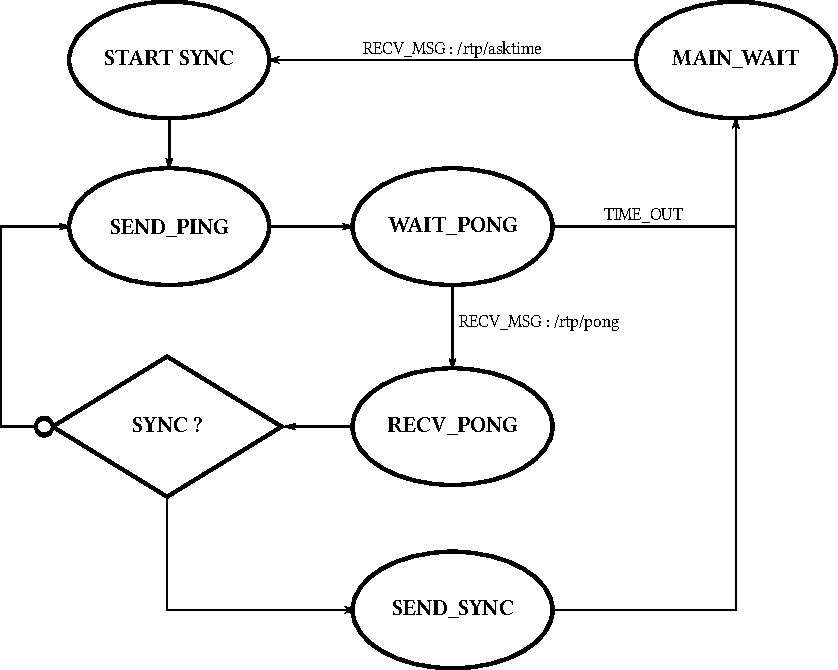
\includegraphics[width=0.95\textwidth]{figs/fsm_time_ref.pdf}
  \caption{FSM de la synchronisation du temps côté référence}
  \label{fig:fsm_time_ref}
  \vspace{-17pt}
\end{figure}~\\

\subsubsection{FSM d'une demande de synchronisation du temps}
Les états de la FSM demandant une synchronisation du temps sont le suivants :
\begin{itemize}
\item \textbf{MAIN\_WAIT} : État d'attente principale du protocole.
\item \textbf{ASK\_SYNC} : Envoie d'un message \textbf{asktime} à une référence.
\item \textbf{WAIT\_PING} : État d'attente après l'envoie d'un \textbf{pong} ou après la demande de synchronisation.
\item \textbf{SEND\_PONG} : Envoie d'un message \textbf{pong} en réponse à un \textbf{ping}
\item \textbf{RECV\_PONG} : État de réception d'un \textbf{pong} et de calcul du temps de parcours puis de l'éventuelle synchronisation
\item \textbf{SYNC\_TIME} : État faisant suite à la réception d'un message \textbf{sync} synchronisant le temps en fonction des valeurs reçues. 
\end{itemize}~\\
La FSM représentant le fonctionnement est la suivante :~\\
\begin{figure}[htbp]
  \centering
  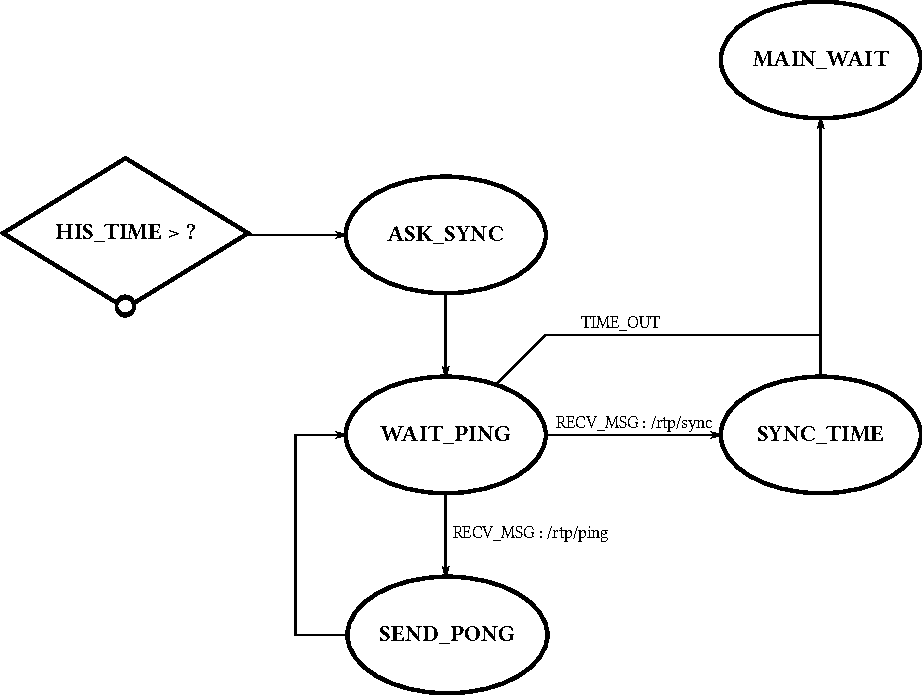
\includegraphics[width=0.95\textwidth]{figs/fsm_sync_ask.pdf}
  \caption{FSM d'une demande de synchronisation du temps}
  \label{fig:fsm_time_ref}
  \vspace{-17pt}
\end{figure}~\\

\subsection{Synchronisation du scénario}


   
\newpage
%\section{Annexes}
%	\subsection{Bibliographie}
% \def\refname{}%
\nocite{*}
%\bibliographystyle{plain-url}
%\bibliography{finite_state_machine}
\printbibliography
%\newpage\textsc{•}


\end{document}